\documentclass[11pt, a4paper]{article}


\usepackage{amsmath,amsfonts,amssymb,amsthm,mathtools}


\usepackage{fontspec}         % пакет для подгрузки шрифтов
\setmainfont{Roboto}          % задаёт основной шрифт документа

\usepackage{unicode-math}     % пакет для установки математического шрифта
\setmathfont{Asana Math}      % шрифт для математики

\usepackage{polyglossia}      % Пакет, который позволяет подгружать русские буквы
\setdefaultlanguage{russian}  % Основной язык документа
\setotherlanguage{english}    % Второстепенный язык документа

\usepackage{graphics}

\usepackage[inline]{enumitem}

\author{Тимур Шакуров}
\title{Первое д.з.}
\date{11.02.17}

\begin{document}

\maketitle

\section{10 фактов обо мне}

\begin{enumerate}

\item Первая книга: "Хоббит, или Туда и Обратно" Толкиена.

\item Умею играть на гитаре, хотя мои соседи оспаривают этот факт

\item Все мои переломы костей(три)происходили по абсолютно нелепым причинам


\end{enumerate}

\section{Фото}

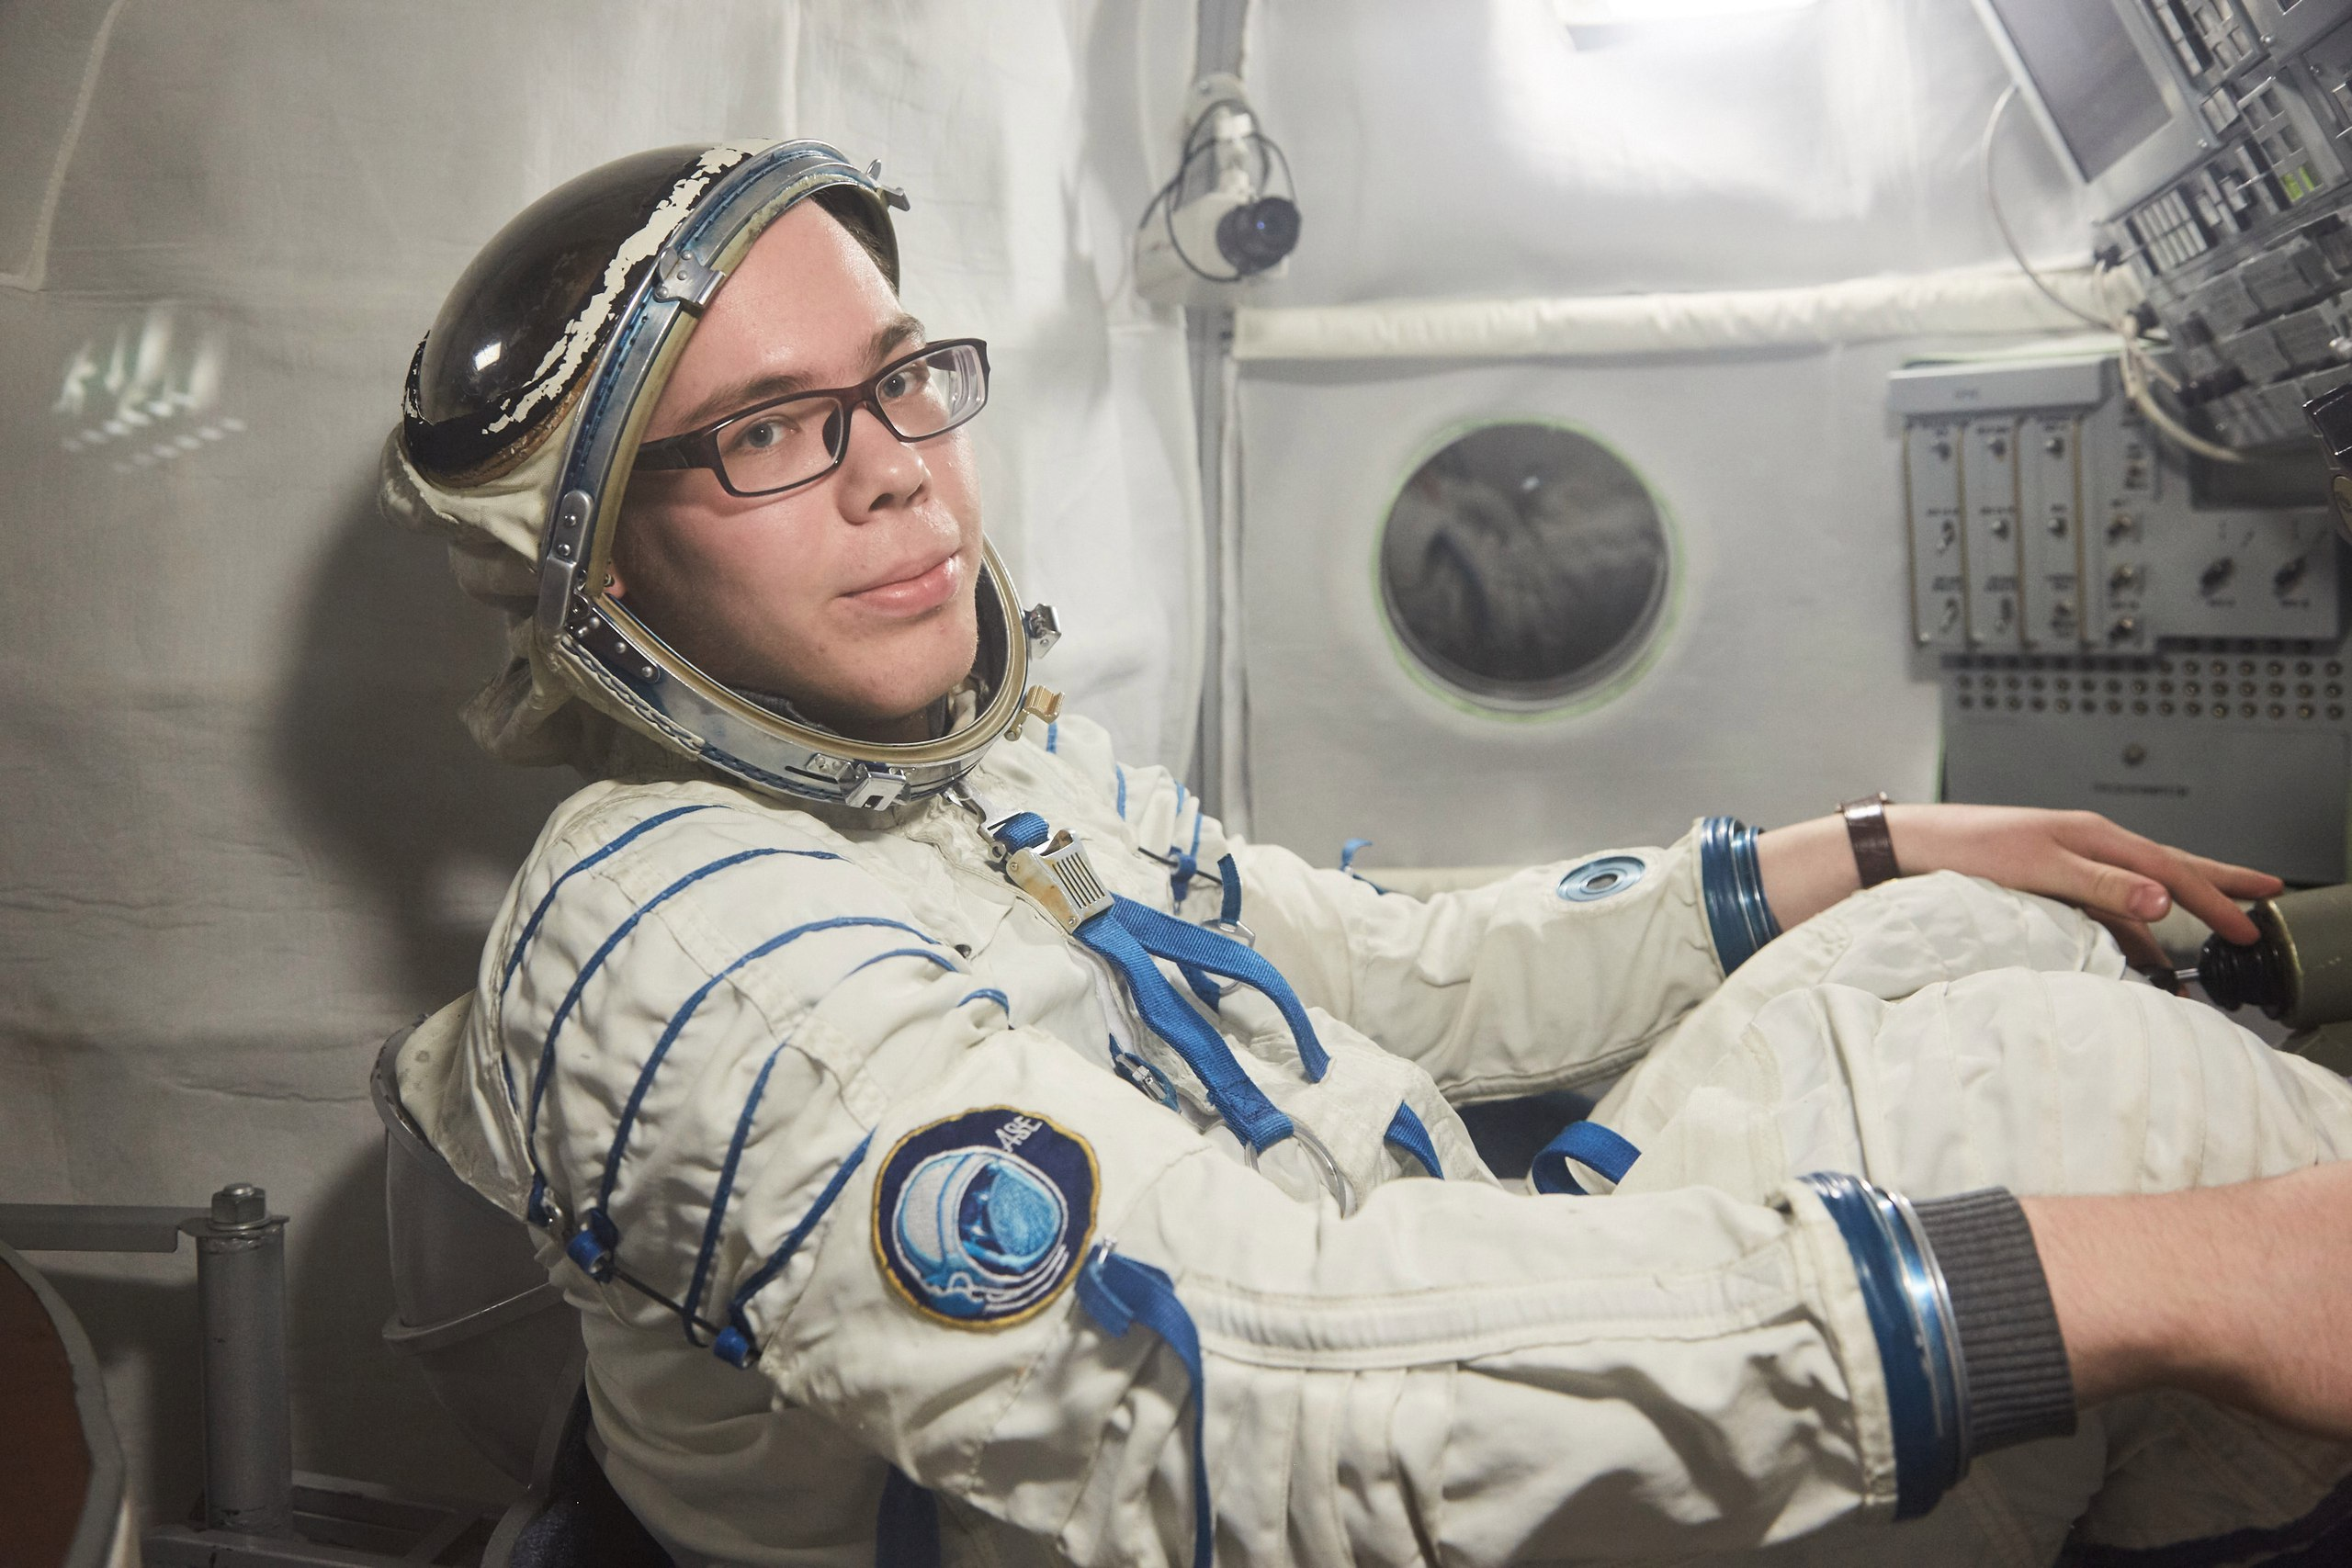
\includegraphics[scale=0.5]{me.jpg}

\section{5 любимых формул}

\begin{enumerate}[label=\setcounter:{what's going on??}] 
\item [æ] $C_n^m=\frac{n!}{(m!(n-m)!}$ \label{f1}

\item [ææ] $\hat{b}_1=\frac{\displaystyle\sum_{i=1}^n (x_i-\bar{x})(y_i-\bar{y})}{\displaystyle\sum_{i=1}^n  (x_i-\bar{x})^2}, \hat{b}_0=\bar{y}-\hat{b}_1\bar{x}$ \label{f2} 
\item [æææ] $det(A)=\begin{vmatrix}
 	a_{1,1} & a_{1,2} \\
 	a_{2,1} & a_{2,2}
\end{vmatrix} = a_{1,1}a_{2,2}-a_{2,1}a_{1,2}$ \label{f3}
\item [ææææ] $\lim_{n \to \infty} P(|\frac{m}{n}-p|<\varepsilon)=1$ \label{f4}
\item [ææææææ] Лемма Ито: $Y_t=f(W_t,t);  f'_t,f''_{W_tW_t} - \text{ непрерывны}, то: Y_t=Y_0+\int_0^t f'_w(W_u,u)dW_u + \int_0^t f'_u (W_u,u)du + \int_0^t f''_{W_uW_u}(W_u,u) du$\label{f5}

\end{enumerate}


\section{Поясняю за формулы}

%Не получилось сослаться на формулы
Формула æ так часто встречается в жизни, что волей-неволей начинаешь ее любить.

Формула ææ - как можно не любить оценку коэффициентов, линейную по Y?  

В случае формулы æææ - определитель матрицы (2 на 2, в данном случае)- мне нравится не столько сама формула, сколько интерпетация - определитель равен площади параллелограмма, образованного векторами - сторонами параллелограмма. 

Формула ææææ - один из главных выводов теории вероятностей. Благодаря ей мы можем изучать генеральные совокупности с помощью выборок и проверять гипотезы.

Лемма Ито - формула æææææ - используется в модели Блэка-Шоулза. Первые шаги в мир оценки стоимости опционов.

\end{document}